\documentclass[tikz]{standalone}

%% pdflatex file
%% pdf2svg triangle.pdf triangle.svg 

\usepackage{standalone}

\begin{document}

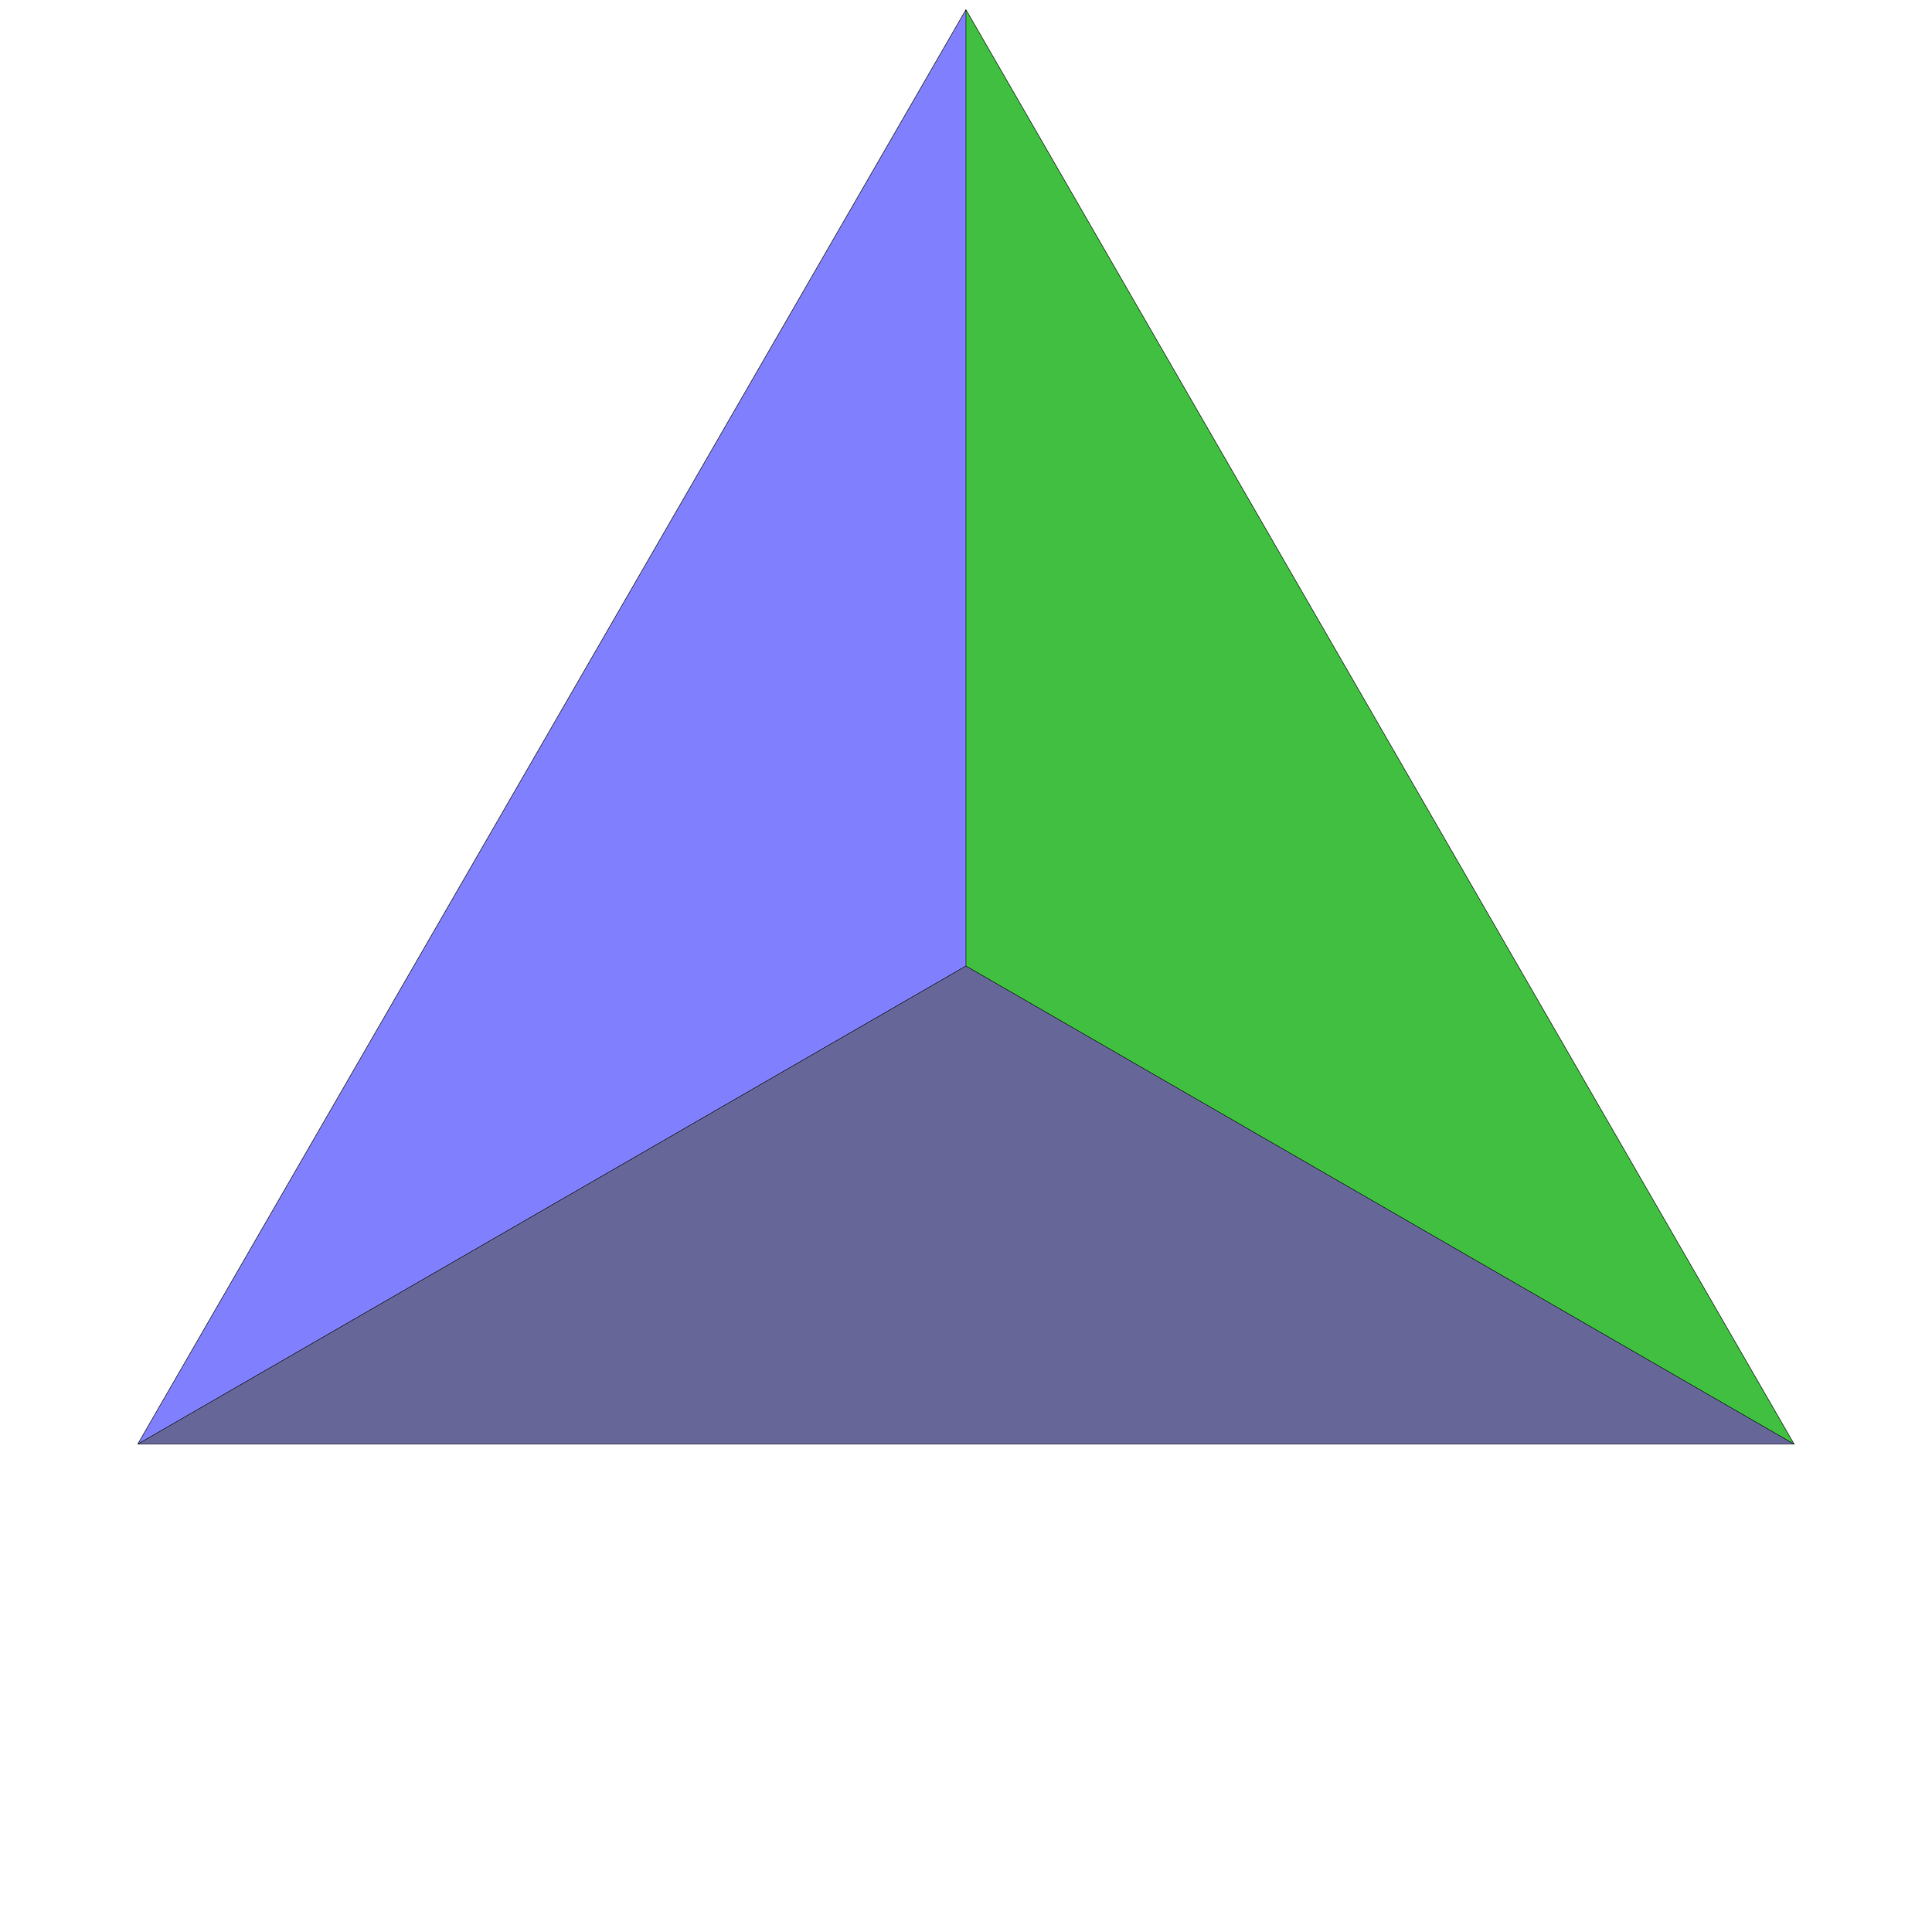
\begin{tikzpicture}[x=1cm,y=1cm] 
  \begin{scope}
    \clip(-34.641,-34.641) rectangle (34.641,34.641);
    \draw[fill=blue,draw=black] (-30,-17.3205) -- (30,-17.3205) -- (0,34.641) -- (-30,-17.3205);

    \draw[fill=blue!20!gray,draw=black] (-30,-17.3205) -- (30,-17.3205) -- (0,0) -- (-30,-17.3205);


    \draw[fill=blue!50!white,draw=black] (-30,-17.3205) -- (0,34.641) -- (0,0) -- (-30,-17.3205);

    \draw[fill=green!50!gray,draw=black] (0,0) -- (0,34.641) -- (30,-17.3205) -- (0,0);

    %\draw (-34.641,-34.641) -- (34.641,34.641);
    %\draw (34.641,-34.641) -- (-34.641,34.641);
  \end{scope}
  \end{tikzpicture}
\end{document}

